\documentclass{article}
\usepackage{enumerate}
\usepackage{algpseudocode}
\usepackage[ruled]{algorithm}
\usepackage{url}
\usepackage{framed}
\usepackage{amsfonts,amsmath,amsthm,amssymb}
\usepackage{graphicx}
\usepackage{url}
\usepackage{color}
\usepackage{geometry}

\geometry{margin=1.2in}

\newcommand {\mean} {\ensuremath {\mathop{\mathrm{mean}}}}
\newcommand {\median} {\ensuremath {\mathop{\mathrm{median}}}}
\newcommand {\N} {\ensuremath {\mathcal{N}}}
\newcommand {\IE} {\ensuremath {\mathbb{E}}}
\newcommand {\cov} {\ensuremath {\mathop{\mathrm{cov}}}}
\newcommand {\BEL} {\ensuremath {\mathop{\mathrm{BEL}}}}

\newtheorem{dfn}{Definition}
\newtheorem{thm}{Theorem}
\newtheorem{lmm}{Lemma}
\newtheorem{crl}{Corollary}

\title{VOI-aware Monte-Carlo Sampling in Trees}
\author {David Tolpin, Solomon Eyal Shimony \\
Department of Computer Science, \\
Ben-Gurion University of the Negev, Beer Sheva, Israel \\
\{tolpin,shimony\}@cs.bgu.ac.il}

\begin{document}

\maketitle

\begin{abstract}
Upper bounds for the VOI are provided for pure exploration in the
Multi-armed Bandit Problem. Sampling policies based on the upper
bounds are suggested. Empirical evaluation of the policies and
comparison to the UCB1 and UCT policies is provided
on random problem instances as well as on the Go game.
\end{abstract}


\section{Introduction and Definitions}

Taking a sequence of samples in order to minimize the
regret of a decision based on the samples is abstracted by the
{\em Multi-armed Bandit Problem.} In the Multi-armed Bandit problem
we have a set of $K$ arms. Each arm can be pulled multiple
times. When the $i$th arm is pulled, a random reward $X_i$ from an
unknown stationary distribution is returned.  The reward is bounded
between 0 and 1.

The simple regret of a sampling policy for the Multi-armed Bandit
Problem is the expected difference between the best expected reward
$\max\limits_i\IE[X_i]$ and the expected reward $\IE[X_j]$ of the arm
with the best sample mean $\overline X_j=\max\limits_i\overline X_i$:
\begin{equation}
\label{eqn:simple-regret}
\IE[R]=\sum_{j=1}^K\Delta_j\Pr(\overline X_j=\max_i\overline X_i)
\end{equation}
where $\Delta_j=\max\limits_i\IE[X_i]-\IE[X_j]$.  Strategies that
minimize the simple regret are called pure exploration strategies
\cite{Bubeck.pure}. Principles of rational metareasoning
\cite{Russell.right} suggest that at each step the arm with the
greatest value of information (VOI) estimate must be pulled, and the
sampling must be stopped and a decision must be made when no arm has
positive VOI estimate.

In order to estimate the VOI of pulling an arm, a sampling model is needed.
The generic sampling model used is: the actual value of an arm has a certain distribution.
Pulling an arm is an i.i.d. noisy measurement of the actual value of the arm.
In \cite{HayRussell.MCTS}, Section 4, two instances of this model are
examined:
\begin{enumerate}[a)]
\item uniformly distributed prior of the value, with Bernouli
  sampling, and 
\item normally distributed prior of the value, with normally
  distributed sampling.
\end{enumerate}

Here we examine the same general setting (i.i.d. samples), but instead
of using a specific distribution model, use {\em concentration
  inequalities} to derive distribution-independent bounds on the
VOI. Our bounds are applicable to any distribution that conforms to
our assumptions, including the case of normally distributed prior of
the value, with normally distributed sampling.

\section{Related Work}

Efficient algorithms for Multi-Armed Bandits based on
distribution-independent bounds, in particular UCB1, are introduced in
\cite{Auer.ucb}. The UCT algorithm, an extension of UCB1 to
Monte-Carlo Tree Search is described in \cite{Kocsis.uct}, and a successful
application of UCT to playing the Go game is discussed in
\cite{Gelly.mogo}.

Pure exploration in Multi-armed bandits is explored in
\cite{Bubeck.pure}. On the one hand, the paper proves certain upper
and lower bounds for UCB1 and uniform sampling, showing that an upper
bound on the simple regret is exponential in the number of samples for
uniform sampling, while only polynomial for UCB1. On the other hand,
empirical performance of UCB1 appears to be better than of uniform
sampling. \cite{Mnih.bernstop} investigate stopping criteria for
sampling based on the empirical Bernstein inequality; however, the
stopping criteria are based on error probabilities rather than on
value of information measures, and do not directly address the
objective of regret minimization.

The principles of bounded rationality appear in
\cite{Horvitz.reasoningabout}. \cite{Russell.right} provided a formal
description of rational metareasoning and case studies of applications
in several problem domains. One obstacle to straightforward
application of the principles of rational metareasoning to Monte-Carlo
sampling is the metagreedy assumption, according to which samples must
be selected as though at most one sample can be taken before an action
is chosen. In Monte-Carlo sampling, the value of information of any
single sample in a given search state is often zero, so a different
approximating assumption must be used instead.

\section{Some Concentration Inequalities}

Let $X_1, \ldots, X_n$ be i.i.d. random variables with values from $[0,1]$,
$X=\frac 1 n \sum_{i=1}^n X_i$. Then 
\begin{description}
\item[Hoeffding inequality \rm{\cite{Hoeffding.ineq}}:] 
\begin{equation}
\Pr(X-\IE[X] \ge a) \le \exp ( -2a^2n)
\label{eqn:conc-hoeffding}
\end{equation}
\item[Empirical Bernstein inequality \rm{(derived in Appendix~\ref{app:deriv-conc-empbernstein})}:]
\begin{eqnarray}
\Pr(X-\IE[X] \ge a) &\le& 2\exp \left( - \frac {a^2n} {\frac {14} {3}
                          \frac {n} {n-1}a+2\overline\sigma_n^2}\right)\nonumber\\
                    &\le& 2\exp \left( - \frac {a^2n} {10a+2\overline\sigma_n^2}\right)
\label{eqn:conc-empbernstein}
\end{eqnarray}
where sample variance $\overline\sigma_n^2$ is
\begin{equation}
\overline\sigma_n^2=\frac 1 {n(n-1)} \sum_{1\le i < j\le n}(X_i-X_j)^2
\label{eqn:sample-variance}
\end{equation}
\end{description}
Bounds (\ref{eqn:conc-hoeffding}, \ref{eqn:conc-empbernstein}) are symmetrical
around the mean. Bound~(\ref{eqn:conc-empbernstein}) is tighter than
(\ref{eqn:conc-hoeffding}) for small $a$ and $\overline\sigma_n^2$. 

\section{Upper Bounds on Value of Information}

The intrinsic VOI $\Lambda_i$ of pulling an arm is the expected decrease
in the regret compared to selecting an arm without pulling any arm at
all. The \textit{myopic} VOI estimate is of limited applicability to
Monte-Carlo sampling, since the effect of a single sample is small,
and the myopic VOI estimate will often be zero, resulting in premature
termination of the search. However, $\Lambda_i$ can be estimated as the intrinsic 
value of perfect information $\Lambda_i^p$ about the mean reward of the $i$th arm. Two
cases are possible:
\begin{itemize}
\item the arm $\alpha$ with the highest sample mean is pulled, and the 
actual arm value is lower than the sample mean of the second-best arm $\beta$;
\item another arm is pulled, and the actual arm value is higher
than the sample mean of the best arm $\alpha$.
\end{itemize}
$\Lambda_i^p$ can be bounded from above as the probability that a
different arm is selected, multiplied by the
maximum possible increase in the reward:
\begin{thm} The intrinsic value of perfect information $\Lambda_i^p$ about the $i$th arm is
  bounded from above as
\begin{equation}
  \Lambda_i^p \le \left\{
  \begin{array}{l l}
    \overline X_\beta \Pr(\IE[X_i] \le \overline X_\beta) & \mbox{{\rm if} $i=\alpha$} \\
    (1-\overline X_\alpha)\Pr(\IE[X_i] \ge \overline X_\alpha) & \mbox{\rm otherwise}
  \end{array} \right.
\label{eqn:thm-vopi}
\end{equation}
\label{thm:vopi}
\end{thm}

\begin{proof} For the case $i\ne \alpha$, the probability that the perfect
  information about the $i$th arm changes the final choice is
  $\Pr(\IE[X_i] \ge \overline X_\alpha)$. $\IE[X_i] \le 1$ by definition,
  therefore the maximum increase in the expected reward is
  $(1-\overline X_\alpha)$. Thus the intrinsic value of perfect
  information is at most $\Pr(\IE[X_i] \ge \overline
  X_\alpha)(1-\overline X_\alpha)$.
  Proof for the case $i=\alpha$ is similar.
\end{proof}

The search time is finite, and in a simple case the \textit{search
  budget} is specified as the maximum number of samples.
An estimate based on the perfect intrinsic VOI does not take in
consideration the remaining number of samples. Given two arms
with the same intrinsic perfect VOI, the VOI
estimate of the arm pulled fewer times so far should be higher.

\begin{dfn} The \textbf{blinkered estimate} of intrinsic VOI information of the
  $i$th arm is the intrinsic VOI of pulling the $i$th arm for the
  remaining budget.
\end{dfn}

\begin{thm} Denote the current number of samples of the $i$th arm by
  $n_i$. The blinkered estimate $\Lambda_i^b$ of intrinsic value of
  information of pulling the $i$th arm for the remaining budget of $N$
  samples is bounded from above as
\begin{equation}
  \Lambda_i^b \le \left\{
  \begin{array}{l l}
    \overline X_\beta\frac N {N+n_i}\Pr(\overline X_i'\le\overline X_\beta)
    \le N\frac {\overline X_\beta} {n_i}\Pr(\overline X_i'\le\overline X_\beta) & \mbox{{\rm if} $i=\alpha$} \\
    (1-\overline  X_\alpha)\frac N {N+n_i}\Pr(\overline X_i'\ge\overline X_\alpha)
       \le N\frac {(1-\overline  X_\alpha)} {n_i}\Pr(\overline X_i'\ge\overline X_\alpha) & \mbox{\rm otherwise}
  \end{array} \right.
\label{eqn:thm-be}
\end{equation}
where $\overline X_i'$ is the sample mean of the $i$th arm after $n_i+N$ 
samples.
\label{thm:be}
\end{thm}

\begin{proof}
The proof is similar to the proof of Theorem~\ref{thm:vopi}, with
$\overline X'_i$ substituted instead of $\IE[X_i]$, and, if
$i\ne\alpha$, an upper bound on $X_i'$ is $X_\alpha+(1-X_\alpha)
\frac N {N+n_i}$; if $i=\alpha$, a lower bound on $X_i'$ is
$X_\beta - X_\beta \frac N {N+n_i}$.
\end{proof}

The probabilities in equations (\ref{eqn:thm-vopi}, \ref{eqn:thm-be})
can be bounded from above using concentration inequalities. In
particular, Theorem~\ref{thm:hoeffding-prob-bounds} (proved in 
Appendix~\ref{app:hoeffding-prob-bounds-proof}) is based on the
Hoeffding inequality (\ref{eqn:conc-hoeffding}):
\begin{thm} The probabilities in equations (\ref{eqn:thm-vopi},
\ref{eqn:thm-be}) are bounded from above as
\begin{eqnarray}
\Pr(\IE[X_i] \le \overline X_\beta|i=\alpha)&
   \le & \exp(-2 (\overline X_i - \overline X_\beta)^2 n_i)\nonumber\\
\Pr(\IE[X_i] \ge \overline X_\alpha|i\ne\alpha)&
   \le & \exp(-2 (\overline X_\alpha - \overline X_i)^2 n_i)
\label{eqn:probound-perf-hoeffding}
\end{eqnarray}
\vspace{-1.5\baselineskip}
\begin{eqnarray}
\Pr(\overline X_i' \le \overline X_\beta|i=\alpha) &
   \le & 2\exp\left(- 2\left(\frac {1+\frac {n_i} N} {1+\sqrt {\frac {n_i} N}}(\overline X_i - \overline X_\beta)\right)^2 n_i \right)
   \le 2\exp\left(- 1.37(\overline X_i - \overline X_\beta)^2 n_i \right) \nonumber\\
\Pr(\overline X_i' \ge \overline X_\alpha|i\ne\alpha) &
   \le & 2\exp\left(- 2\left(\frac {1+\frac {n_i} N} {1+\sqrt {\frac {n_i} N}} (\overline X_\alpha - \overline X_i)\right)^2 n_i \right)
    \le 2\exp\left(- 1.37(\overline X_\alpha - \overline X_i)^2 n_i \right)
\label{eqn:probound-blnk-hoeffding}
\end{eqnarray}
\label{thm:hoeffding-prob-bounds}
\end{thm}

\begin{crl} An upper bound on the intrinsic value of perfect information is obtained by substituting
(\ref{eqn:probound-perf-hoeffding}) into (\ref{eqn:thm-vopi}):
\begin{equation}
  \Lambda_i^p \le \hat\Lambda_i^p=\left\{
  \begin{array}{l l}
    \overline X_\beta\cdot \exp\left(- 2(\overline X_i - \overline X_\beta)^2 n_i \right) & \mbox{{\rm if} $i=\alpha$} \\
    (1-\overline  X_\alpha)\cdot \exp\left(- 2(\overline X_\alpha - \overline X_i)^2 n_i \right)  &  \mbox{\rm otherwise}
  \end{array} \right.
\label{eqn:bound-perf-hoeffding}
\end{equation}
\label{crl:bound-perf-hoeffding}
\end{crl}
\begin{crl}
An upper bound on the blinkered VOI estimate with ordering independent of $N$ is obtained
by substituting (\ref{eqn:probound-blnk-hoeffding}) into (\ref{eqn:thm-be}).
\begin{equation}
  \Lambda_i^b \le \hat\Lambda_i^b=\left\{
  \begin{array}{l l}
    N\frac {\overline X_\beta} {n_i}\cdot 2\exp\left(- 1.37(\overline X_i - \overline X_\beta)^2 n_i\right)
      & \mbox{{\rm if} $i=\alpha$} \\
    N\frac {(1-\overline  X_\alpha)} {n_i}\cdot 2\exp\left(- 1.37(\overline X_\alpha - \overline X_i)^2 n_i\right)
      &  \mbox{\rm otherwise}
  \end{array} \right.
\label{eqn:bound-blnk-hoeffding}
\end{equation}
\label{crl:bound-blnk-hoeffding}
\end{crl}
Bound~\ref{eqn:bound-blnk-hoeffding} is generally tighter when $N$ is
small relative to $n_i$. Estimate $\hat\Lambda_i^b$ can be viewed as a
relaxation of the myopic assumption such that sequences consisting
of more than one action are taken into considertion. Better bounds can
be obtained through tighter estimates on the probabilities, for
example, based on the empirical Bernstein inequality
(\ref{eqn:conc-empbernstein}) or through a more careful application of
the Hoeffding inequality (Appendix~\ref{app:better-hoeffding-bound}).

\section{VOI-based Sampling Control}

\subsection{Selection Criterion}

Following the principles of rational metareasoning, an arm with
the highest VOI should be pulled at each step. The upper bounds
established in Theorems~\ref{thm:vopi},~\ref{thm:be} can be used
as VOI estimates. Blinkered VOI estimates~(\ref{eqn:thm-be},
 \ref{eqn:bound-blnk-hoeffding}) can be viewed
as approximations of VOI estimates for myopic or
receding horizon policies. As illustrated by the empirical evaluation
(Section~\ref{sec:empirical-evaluation}), estimates based on upper
bounds on the VOI result in rational sampling policies, and exhibit
performance comparable to the performance of some state-of-the-art
heuristic algorithms.

\subsection{Termination Condition}
\label{sec:control-termination-condition}

The simplest termination condition for a sampling policy is the
budget---a fixed number of samples performed before a decision is
made. When a sample has a cost commensurable with the value of
information of a measurement, an upper bound on the intrinsic VOI can
be used to stop the sampling if the intrinsic VOI of any action
is less than the cost of sampling $C$:
\begin{equation}
\mbox{stop if } \max_i \Lambda_i \le C
\end{equation}
Blinkered VOI estimates~(\ref{eqn:thm-be},
\ref{eqn:bound-blnk-hoeffding}) include the remaining budget $N$ as a
factor, but given the cost of a single sample $c$, the cost of the
remaining samples accounted for in estimating the intrinsic VOI is
$C=cN$. $N$ can be dropped on both sides of the inequality,
and a viable stopping condition is
\begin{equation}
\begin{array}{c r r l l}
&\frac 1 N \Lambda_\alpha^b
\le\frac {\overline  X_\beta} {n_\alpha}\Pr(\overline X_\alpha'\le\overline X_\beta)&\le& c
&\nonumber\\
\mbox{and}&&&&\nonumber\\
&\frac 1 N \max_i\Lambda_i^b
\le \max_i\frac {(1-\overline  X_\alpha)} {n_i}\Pr(\overline X_i'\ge\overline X_\alpha)&\le& c
 & \forall i: i\ne\alpha
\end{array}
\label{eqn:stopping-blnk}
\end{equation}
The empirical evaluation (Section~\ref{sec:empirical-evaluation})
confirms viability of this stopping condition and illustrates the
influence of the sample cost $c$ on the performance of
the sampling policy.

\subsection{Sample Redistribution in Trees}
\label{sec:control-redistribution}

Monte-Carlo tree search \cite{Chaslot.montecarlo} selects at each
search step an action that appears to be the best based on outcomes
of \textit{search rollouts}. Two different criteria are employed in
action selection during a rollout:
\begin{itemize}
\item at the first step, the value of partial
information should be maximized to minimize the \textit{simple} regret
of the selection at the current root node;
\item as the goal of sampling in deeper tree nodes is estimating the
value of a node, rather than selection, it makes sense to minimize
the \textit{cumulative} regret of the rollouts from the second step
onwards.
\end{itemize}

A natural approach would be to apply an algorithm that minimizes the
simple regret in Multi-armed bandits at the first step, and the
cumulative regret during the rest of the rollout.  However, this
approach assumes that the information obtained from rollouts in the
current state is discarded after an action is selected. In practice,
many successful Monte-Carlo tree search algorithms re-use rollouts
originating from an earlier search state and passing through the
current search state; thus, the value of information of a rollout is
determined not just by the influence on the choice of the action at
the current state, but also by the influence on the choice at future
search states, provided the rollout passes through the search states
which will be visited.

One way to account for this re-use would be to incorporate the
`future' value of information into a VOI estimate. However, this 
approach appears to be complicated. Alternatively, one can behave
myopically in search tree depth:
\begin{enumerate}
\item estimate VOI as though the information is discarded after each step;
\item stop early if the VOI is below a certain threshold
   (see Section~\ref{sec:control-termination-condition});
\item save the unused sample budget for search in future state, such that
   if the nominal budget is $N$, and the unused budget in the last state
   is $N_u$, the search budget in the next state will be $N+N_u$.
\end{enumerate}
In this approach, the cost of a sample in the current state is the
VOI of increasing the budget of a future state by one sample.  It is
unclear whether this cost can be accurately estimated, but supposedly
a fixed value for a given problem type and algorithm implementation
would work. Indeed, the empirical evaluation (Section~\ref{sec:emp-go})
confirms that stopping and sample redistribution based on a learned
fixed cost  substantially improve the performance of the VOI-based
sampling policy in game tree search.

\section{Empirical Evaluation}
\label{sec:empirical-evaluation}

The experiments compare the UCT algorithm \cite{Kocsis.uct} with
modified versions of UCT in which the samples at the first step are
selected according to their VOI estimates. Three blinkered VOI
estimates were used for the comparison:
\begin{description}
\item[VCT:] based on Hoeffding inequality (\ref{eqn:conc-hoeffding});
\item[ECT:] based on Hoeffding inequality with an intermediate point (see
Appendix~\ref{app:better-hoeffding-bound});
\item[BCT:] based on empirical Bernstein inequality
(\ref{eqn:conc-empbernstein}).
\end{description}
For simplicity, the bounds on probability for an unlimited number
of samples were used in the estimate formulas. The estimates where
computed as follows:
\begin{eqnarray}\
  \Lambda_i^{VCT}& =&\left\{
  \begin{array}{l l}
    \frac {\overline X_\beta} {n_i} \cdot \exp\left(- 2(\overline X_i - \overline X_\beta)^2 n_i\right)
      & \mbox{{\rm if} $i=\alpha$} \\
    \frac {(1-\overline  X_\alpha)} {n_i}\cdot \exp\left(- 2(\overline X_\alpha - \overline X_i)^2 n_i\right)
      &  \mbox{\rm otherwise}
  \end{array}  \right.\nonumber\\
  \Lambda_i^{ECT}& =&\min\left(\Lambda_i^{VCT}, \min_y\left\{
  \begin{array}{l l}
    \frac {\overline X_\beta-y} {n_i}\cdot \exp\left(-2 (\overline X_i-\overline X_\beta)^2n_i\right)
    +\frac {\overline X_\beta} {n_i}\cdot \exp\left(-2 (\overline X_i-y)^2n_i\right)
      & \mbox{{\rm if} $i=\alpha$} \\
\frac {y-\overline X_\alpha} {n_i}\cdot \exp\left(-2(\overline X_\alpha-\overline X_i)^2n_i\right)
    +\frac {1-\overline X_\alpha} {n_i}\cdot \exp\left(-2 (y-\overline X_i)^2n_i\right)
      &  \mbox{\rm otherwise}
  \end{array} \right.\right) \nonumber\\
  \Lambda_i^{BCT}& =&\min\left(\Lambda_i^{VCT},\left\{
  \begin{array}{l l}
    \frac {\overline X_\beta} {n_i}\cdot 2\exp\left(- \frac {(\overline X_i - \overline X_\beta)^2 n_i} {\frac {14} 3 \frac {n_i} {n_i-1}(\overline X_i - \overline X_\beta) + 2 \overline X_i(1-\overline X_i)} \right)
      & \mbox{{\rm if} $i=\alpha$} \\
    \frac {(1-\overline  X_\alpha)} {n_i}\cdot 2\exp\left(- \frac {(\overline X_\alpha - \overline X_i)^2 n_i} {\frac {14} 3 \frac {n_i} {n_i-1}(\overline X_\alpha - \overline X_i) + 2 \overline X_i(1-\overline X_i)} \right)
      &  \mbox{\rm otherwise}
  \end{array} \right.\right)
\label{eqn:emp-estimates}
\end{eqnarray}

\subsection{Selecting The Best Arm}
\label{sec:emp-arm}

\begin{figure}[t]
\centering
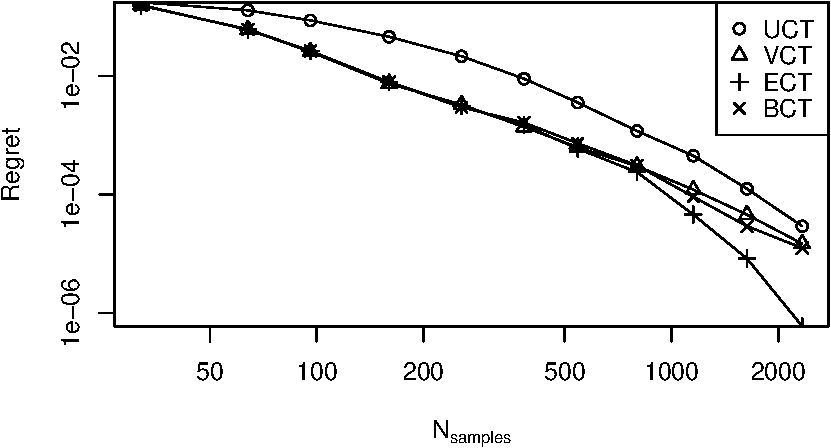
\includegraphics[scale=0.8]{flat.pdf}
\caption{Random instances: regret vs. number of samples}
\label{fig:random-instances}
\end{figure}

The sampling policies are first compared on random Multi-armed bandit 
problem instances, where the Monte-Carlo Tree Search algorithm
is reduced to the sample selection policy at the first step: UCT is 
actually UCB1. In the problem of pure exploration in Multi-armed bandits
\cite{Bubeck.pure}, the smaller the exploration factor, the higher
the expected simple regret is; indeed, UCT exhibits the lowest simple
regret in the experiments for the default exploration factor $Cp=\frac
{\sqrt 2} 2$ \cite{Kocsis.uct}.

Figure~\ref{fig:random-instances} shows experiment results for
randomly-generated Multi-armed bandits with 32 Bernoulli arms, with
the mean rewards of the arms distributed uniformly in the range $[0,
  1]$, for a range of sample budgets $32..2048$, with multiplicative
step of $2$. The experiment for each number of samples was repeated
20000 times. UCT is worse than any of the VOI-aware sampling policies,
for example, for 384 samples the simple regret of UCT is $\approx 40$
times greater than of VCT, and $\approx 100$ times greater than of
ECT. On average, it takes $2.5$ times as many samples for UCT to reach
the regret of VCT. Different numbers of arms and distributions of
means give similar results.

\subsection{Playing Go Against UCT}
\label{sec:emp-go}

One search domain in which Monte-Carlo tree search based on the UCT
sampling policy has been particularly successful is playing the game Go
\cite{Gelly.mogo}. This series of experiments compares
the winning rate of UCT against VOI-aware policies (VCT, ECT, BCT)
in Go and investigates the effect of early stopping and sample
redistribution. 

For the experiments, a modified version of Pachi \cite{Braudis.pachi},
a state of the art Go program, was used:
\begin{itemize}
\item The UCT engine of Pachi was extended with VOI-aware sampling
  policies at the first step. 
\item The stopping condition for the VOI-aware policies was
  modified and based solely on the sample cost, specified as
  a constant parameter. 
\item The time-allocation mode based on the fixed number of samples
  was modified such that 
  \begin{enumerate}
    \item the same number of samples is available to
      the agent at each step, independently of the number of pre-simulated
      games;  
    \item if samples were unused at the current step,
      they become available at the next step.
  \end{enumerate}
\end{itemize}
While the UCT engine is not the most powerful engine of Pachi, it is still
a strong player. On the other hand, additional
features of more advanced engines would obstruct the Monte-Carlo
sampling phenomena which are the subject of the experiment.

\begin{figure}[t]
\centering
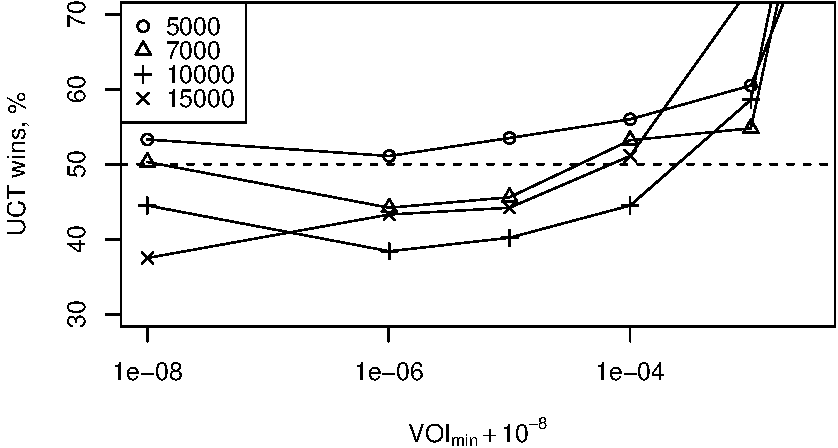
\includegraphics[scale=0.8]{vct-wins.pdf}
\caption{Go: winning rate --- UCT against VCT}
\label{fig:uct-against-vct}
\end{figure}
\begin{figure}[t]
\centering
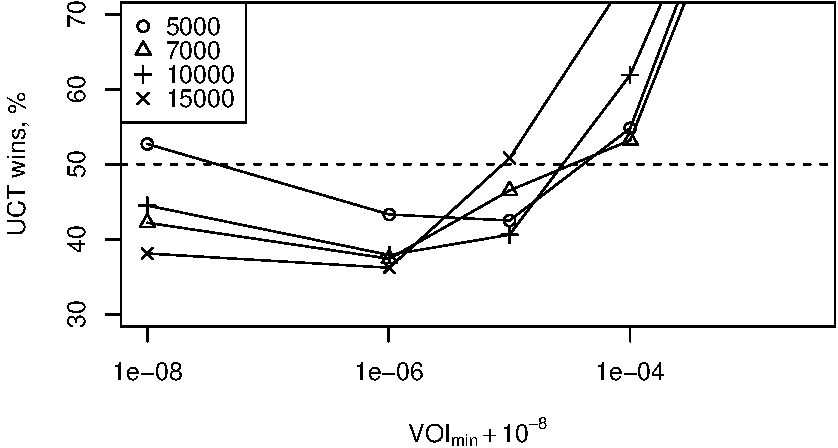
\includegraphics[scale=0.8]{ect-wins.pdf}
\caption{Go: winning rate --- UCT against ECT}
\label{fig:uct-against-ect}
\end{figure}
\begin{figure}[t]
\centering
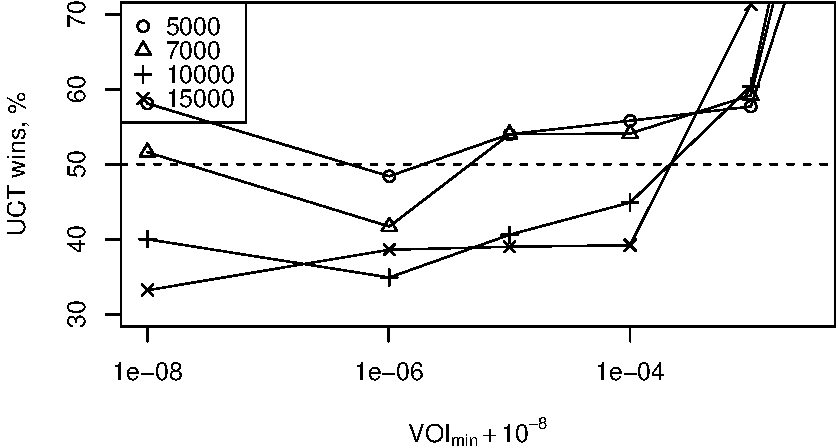
\includegraphics[scale=0.8]{bct-wins.pdf}
\caption{Go: winning rate --- UCT against BCT}
\label{fig:uct-against-bct}
\end{figure}
The engines were compared on the 9x9 board, for 5000, 7000, 1000, and
15000 samples (game simulations) per ply, each experiment was repeated
1000 times. Figures~\ref{fig:uct-against-vct}--\ref{fig:uct-against-bct} show the
winning rate of UCT against VCT, ECT, BCT, correspondingly, vs. the
stopping threshold (if the maximum VOI of a sample is below the
threshold, the simulation is stopped, and a move is chosen). Each curve
in the figures corresponds to a certain number of samples per ply. The
lower the curve, the better is the corresponding policy compared to UCT.

As the results show, without sample redistribution UCT is as good as or
better than the VOI-aware policies for lower numbers of samples per ply
(5000, 7000), and the advantage of VOI-aware policies for larger
number of samples is rather modest (e.g., ECT wins in 55\% of games for
10000 samples per ply). For the stopping threshold of $10^{-6}$,
however, the VOI-aware policies are almost always better than UCT
(only VCT for 5000 samples wins in less than 50\% of games), with
stronger policies (ECT, VCT) reaching the winning rate of 66\%.

In agreement with intuition
(Section~\ref{sec:control-redistribution}), VOI-based stopping and sample
redistribution is most influential for medium numbers of samples per
ply. When the maximum number of samples is too low, early stopping would
result in poorly selected moves. On the other hand, when the maximum
number of samples is sufficiently high, the VOI of increasing the
maximum number of samples in a future state is low.

\begin{figure}[t]
\centering
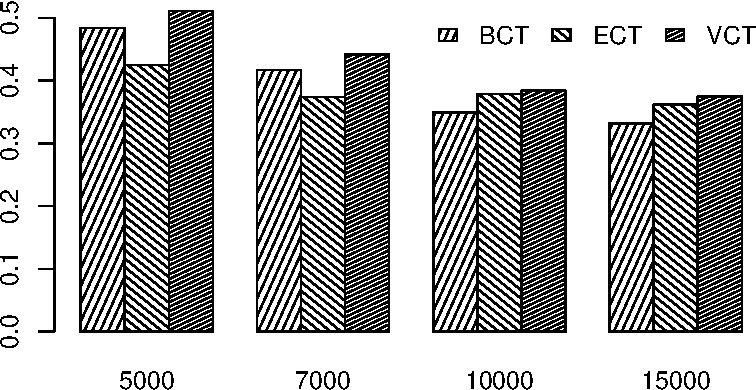
\includegraphics[scale=0.8]{bests-bw.pdf}
\caption{Go: best winning rate comparison}
\label{fig:best-winning-rate}
\end{figure}
Figure~\ref{fig:best-winning-rate} presents relative performance of
different VOI-aware policies depending on the number of samples per
ply by comparing the best achieved winning rates against UCT (again,
the lower the bar, the better is the policy). Both ECT (based on the
Hoeffding inequality with an intermediate point) and BCT (based on the empirical
Bernstein inequality) are better than VCT. The difference between ECT
and VCT is most prominent for smaller number of samples, and the
winning rate of ECT increases relatively slowly with the number of
samples. In contrast, BCT is worse than ECT and only slightly better
than VCT for smaller number of samples, but the winning rate rapidly
increases with the number of samples, and for 10000 and 15000 samples
per ply BCT is the best of the policies with the winning rate reaching
67\%.

\section{Summary and Future Work}

This work suggested Monte-Carlo sampling policies in which sample
selection and termination are based on upper bounds on the value of
information. A simplified model of accounting for future value of
information of a sample, based on early termination and sample
redistribution, was proposed for Monte-Carlo sampling in
trees. Empirical evaluation showed that these policies outperform
heuristic algorithms for simple regret minimization in Multi-armed
bandits, as well as for tree search.

Monte-Carlo tree search still remains a largely unexplored field of
application of VOI-aware algorithms. More elaborated VOI estimates,
taking into consideration re-use of samples in future search states
should be considered. The policies introduced in the paper differ from
the UCT algorithm only at the first step, where the VOI-aware
decisions are made. Consistent application of principles of rational
metareasoning at all steps of a rollout may further improve the
sampling policies.

\section{Proof of Theorem~\ref{thm:hoeffding-prob-bounds}}
\label{app:hoeffding-prob-bounds-proof}

\begin{proof}[]
Equations (\ref{eqn:probound-perf-hoeffding}) is a direct
application of the Hoeffding inequality (\ref{eqn:conc-hoeffding}).

Equations (\ref{eqn:probound-blnk-hoeffding}) follow from the
observation that if $i\ne\alpha$, $\overline X_i'>\overline X_\alpha$
if and only if the mean $\overline X_i^+$ of $N$ samples from $n_i+1$
to $N$ is at least $\overline X_\alpha+(\overline X_\alpha-\overline
X_i)\frac {n_i} N$.

For any $\delta$, the probability that $\overline X_i'$ is greater
than $\overline X_\alpha$ is less than the probability that
$\IE[X_i]\ge\overline X_i+\delta$
\emph{or} $\overline X_i^+\ge \IE[X_i]+\overline X_\alpha
- \overline X_i - \delta +(\overline X_\alpha - \overline X_i)\frac {n_i} N$,
thus, by the union bound, less than the sum of the probabilities:
\begin{equation}
\Pr(\overline X_i'\ge \overline X_\alpha)\le
  \Pr(\IE[X_i]-\overline X_i \ge \delta)+
  \Pr\left(\overline X_i^+ - \IE[X_i] \ge \overline X_\alpha
           - \overline X_i - \delta +(\overline X_\alpha - \overline X_i)\frac {n_i} N\right)
\end{equation}
Bounding the probabilities on the right-hand side using the Hoeffding
inequality, obtain:
\begin{equation}
\Pr(\overline X_i'\ge \overline X_\alpha)\le 
    \exp(-2\delta^2n_i)+
         \exp\left(-2\left((\overline X_\alpha 
         - \overline X_i)\left(1+\frac {n_i} N\right)
         - \delta\right)^2N\right)
\label{eqn:app-hoeffding-le-maxexp}
\end{equation}
Find $\delta$ for which the two terms on the right-hand side of
(\ref{eqn:app-hoeffding-le-maxexp}) are equal:
\begin{equation}
\exp(-\delta^2n) = \exp(-2\left((\overline X_\alpha - \overline X_i)(1+\frac {n_i} N) - \delta\right)^2N)\label{eqn:app-hoeffding-eq-exp}
\end{equation}
Solve (\ref{eqn:app-hoeffding-eq-exp}) for $\delta$: $\delta=\frac {1+\frac {n_i} N} {1+\sqrt {\frac {n_i} N}} (\overline X_\alpha
- \overline X_i) \ge (\sqrt 2 - 1)(\overline X_\alpha-\overline X_i)$. Substitute $\delta$ into 
(\ref{eqn:app-hoeffding-le-maxexp}) and obtain
\begin{eqnarray}
\Pr(\overline X_i'\ge \overline X_\alpha) 
& \le & 2\exp\left(-2\left( \frac {1+\frac {n_i} N} {1+\sqrt {\frac {n_i} N}}
                          (\overline X_\alpha - \overline X_i)\right)^2 n_i\right)\nonumber \\
& \le & 2\exp(-2(\sqrt 2 - 1)^2(\overline X_\alpha - \overline X_i)^2n_i)
 \le 2\exp(-1.37(\overline X_\alpha - \overline X_i)^2n_i)
\end{eqnarray}
Derivation for the case $i=\alpha$ is similar.
\end{proof}

\section{Empirical Bernstein Inequality}
\label{app:deriv-conc-empbernstein}

Theorem~4 in~\cite{MaurerPontil.benrstein} states that
\begin{equation}
\Pr\left(\IE[X]-\overline X_n
    \ge \sqrt { \frac {2\overline\sigma_n^2 \ln 2/\delta} n } + \frac {7 \ln 2/\delta} {3(n-1)}\right)\le \delta
\end{equation}
Therefore
\begin{equation}
\Pr\left(\IE[X]-\overline X_n \ge
              \sqrt { \left(\frac {7 \ln 2/\delta} {3(n-1)}\right)^2+\frac {2\overline\sigma_n^2 \ln 2/\delta} n }
                      + \frac {7 \ln 2/\delta} {3(n-1)}\right)
   \le \delta.
\end{equation}
$a=\sqrt { \left(\frac {7 \ln 2/\delta} {3(n-1)}\right)^2+\frac {2\overline\sigma_n^2 \ln 2/\delta} n } + \frac {7 \ln 2/\delta} {3(n-1)}$
 is a root of square equation $a^2-a\frac {14 \ln 2/\delta} {3(n-1)} -\frac {2\overline\sigma_n^2 \ln 2/\delta} n=0$
which, solved for $\delta\triangleq\Pr(\IE[X]-\overline X_n\ge a)$,
gives
\begin{equation*}
\Pr(\IE[X]-\overline X_n\ge a)\le 2\exp \left( - \frac {na^2} {\frac {14} {3} \frac {n} {n-1}a+2\overline\sigma_n^2}\right)
\end{equation*}
Other derivations, giving slightly different results, are possible.

\section{Better Hoeffding-Based Bound on Value of Perfect Information}
\label{app:better-hoeffding-bound}

Bounds (\ref{eqn:bound-perf-hoeffding}, \ref{eqn:bound-blnk-hoeffding}) have the form
\begin{equation}
  \Lambda_i \le \hat\Lambda_i=\left\{
  \begin{array}{l l}
    (\overline X_\beta-B)\exp\left(- \gamma(\overline X_i - \overline X_\beta)^2 n_i \right) & \mbox{{\rm if} $i=\alpha$} \\
    (A-\overline  X_\alpha)\exp\left(- \gamma(\overline X_\alpha - \overline X_i)^2 n_i \right)  &  \mbox{\rm otherwise}
  \end{array} \right.
\label{eqn:bound-generic-hoeffding}
\end{equation}
where $A$ is the upper bound on the posterior sample mean $\overline
X_i'$ if $i\ne \alpha$, $B$ is the lower bound on $\overline X_i'$ if
$i=\alpha$. For $i=\alpha$, the bound can be improved by selecting an
intermediate point $y$, $B < y < \overline X_\beta$, and computing the bound
as the sum of two parts: 
\begin{itemize}
\item $\overline X_\beta-y$ multiplied by the probability that
  $\overline X_i' \le \overline X_\beta$;
\item $\overline X_\beta-B$ multiplied by the probability that $\overline X_i'\le
  y$.
\end{itemize}.
\begin{equation}
\Lambda_{i|i=\alpha} \le \hat \Lambda_{i|i=\alpha} =
 (\overline X_\beta-y)\exp\left(-\gamma (\overline X_i-\overline X_\beta)^2n_i\right)
 +(\overline X_\beta-B)\exp\left(-\gamma (\overline X_i-y)^2n_i\right)
\label{eqn:bound-twopart-hoeffding-alpha}
\end{equation}
If $y$ that minimizes $\hat\Lambda_{i|i=\alpha}$ exists, the minimum is achieved when
 $\frac {d\hat\Lambda_{i|i=\alpha}} {dy}=0$, that
is, when $y$ is the root of the following equation:
\begin{equation}
  2\gamma (\overline X_\beta-B)(\overline X_i-y)n_i = \exp\left(-\gamma \left(\frac {\overline X_i-\overline X_\beta}
    {\overline X_i-y}\right)^2n_i\right)
\end{equation}
The derivation for the case $i\ne \alpha$ is obtained by substitution $1-A, 1-\overline X_i, 1-\overline X_\alpha, 1-y$ instead of
$B, \overline X_i, \overline X_\beta, y$ into (\ref{eqn:bound-twopart-hoeffding-alpha}):
\begin{equation}
\Lambda_{i|i\ne\alpha} \le \hat\Lambda_{i|i\ne\alpha} = (y-\overline X_\alpha)\exp\left(-\gamma(\overline X_\alpha-\overline
  X_i)^2 n_i\right)+(A-\overline X_\alpha)\exp\left(-\gamma (y-\overline X_i)^2n_i\right)
\label{eqn:bound-twopart-hoeffding-rest}
\end{equation}
A closed-form solution for $y$ cannot be obtained, but given
$A, B, \overline X_\alpha, \overline X_\beta, n$, the value of $y$ can be efficiently
computed.

\bibliographystyle{plain}
\bibliography{refs}

\end{document}
